\documentclass[14pt]{beamer}

\usepackage{xcolor}
\usepackage{colortbl}
\usepackage{pgf}
\usepackage{amsmath}
\usepackage{amssymb}
\usepackage{latexsym}
\usepackage{tikz}
\usepackage{pgfplots}
\usepackage{pdfpages}
\usepackage{ulem}

\definecolor{shaded}{RGB}{210,210,210}
\usecolortheme[named=shaded]{structure}

\definecolor{stressed}{RGB}{150,40,40}
\setbeamercolor{alerted_text}{fg=stressed}


\setbeamertemplate{navigation symbols}{}
\setbeamersize{text margin left=3mm} 
\setbeamersize{text margin right=3mm} 

%\usepackage{fontspec,xunicode,xltxtra}
%\setmainfont{Helvetica Neue Light}
%\setsansfont{Helvetica Neue Light}

%\usepackage[T1]{fontenc}
%\usepackage{tgheros}
%\renewcommand*\familydefault{\sfdefault} %% Only if the base font of the document is to be sans serif

\setbeamertemplate{sidebar right}{default}{}

\makeatletter
\define@key{beamerframe}{nofills}[true]{% top
  \beamer@frametopskip=0pt\relax%
  \beamer@framebottomskip=0pt\relax%
  \beamer@frametopskipautobreak=\beamer@frametopskip\relax%
  \beamer@framebottomskipautobreak=\beamer@framebottomskip\relax%
  \def\beamer@initfirstlineunskip{%
    \def\beamer@firstlineitemizeunskip{%
      \vskip-\partopsep\vskip-\topsep\vskip-\parskip%
      \global\let\beamer@firstlineitemizeunskip=\relax}%
    \everypar{\global\let\beamer@firstlineitemizeunskip=\relax}}
}
\makeatother

\newcommand{\setbackgroundpicturewhite}[1]{%
\usebackgroundtemplate{%
\begin{tikzpicture}%
\draw[fill=white] (current page.north west) rectangle (current page.south east);%
\node[draw,minimum width=\paperwidth,minimum height=\paperheight] [anchor=south west] (mynode) {\includegraphics[width=\paperwidth]{#1}};%
\end{tikzpicture}%
}%
%\begin{pgfpicture}{0in}{0in}{\paperwidth}{\paperheight}
%\pgfputat{\pgfxy(0,0)}{\includegraphics[width=\paperwidth]{#1}}
%\color{white}
%\pgfsetfillopacity{0.0}
%\pgfrect[fill]{\pgfxy(0,0)}{\pgfpoint{\paperwidth}{\paperheight}}
%\end{pgfpicture}
%}
}


\newcommand{\setbackgroundpictureblack}[1]{%
\usebackgroundtemplate{%
\begin{tikzpicture}%
\draw[fill=black] (current page.north west) rectangle (current page.south east);%
\node[draw,minimum width=\paperwidth,minimum height=\paperheight] [anchor=south west] (mynode) {\includegraphics[width=\paperwidth]{#1}};%
\end{tikzpicture}%
}%
%\begin{pgfpicture}{0in}{0in}{\paperwidth}{\paperheight}
%\pgfputat{\pgfxy(0,0)}{\includegraphics[width=\paperwidth]{#1}}
%\color{white}
%\pgfsetfillopacity{0.0}
%\pgfrect[fill]{\pgfxy(0,0)}{\pgfpoint{\paperwidth}{\paperheight}}
%\end{pgfpicture}
%}
}


\newcommand{\setdarkbackgroundpictureblack}[1]{%
\usebackgroundtemplate{%
\begin{tikzpicture}%
\draw[fill=black] (current page.north west) rectangle (current page.south east);%
\node[draw,very thick,minimum width=\paperwidth-\pgflinewidth,minimum height=\paperheight-\pgflinewidth] [anchor=south west] (mynode) {\includegraphics[width=\paperwidth]{#1}};%
\draw[fill=black,opacity=0.75] (current page.north west) rectangle (current page.south east);%
\end{tikzpicture}%
}}%


\newcommand{\setdarkbackgroundpicturewhite}[1]{%
\usebackgroundtemplate{%
\begin{tikzpicture}%
\draw[fill=white] (current page.north west) rectangle (current page.south east);%
\node[draw,very thick,minimum width=\paperwidth-\pgflinewidth,minimum height=\paperheight-\pgflinewidth] [anchor=south west] (mynode) {\includegraphics[width=\paperwidth]{#1}};%
\draw[fill=white,opacity=0.75] (current page.north west) rectangle (current page.south east);%
\end{tikzpicture}%
}}%


\newcommand{\clearbackgroundpicture}{\usebackgroundtemplate{}}

\begin{document}
\setbeamercolor{background canvas}{bg=white,fg=black}
\usebeamercolor[fg]{background canvas}

%%%%%%%%%%%%%%%%%%%%%%%%%%%%%%%%%%%%%%%%%%%%%%%%%%%%%%%%%%%%%%%%
\clearbackgroundpicture
\begin{frame}[nofills]
  \includegraphics[width=\textwidth]{cow.pdf}

  \vfill
  \Large
  \textsf{\textbf{Jim Fowler}} \\
  \textsf{OSU Mathematics Department}
\end{frame}

%%%%%%%%%%%%%%%%%%%%%%%%%%%%%%%%%%%%%%%%%%%%%%%%%%%%%%%%%%%%%%%%
% Coursera
\setbackgroundpicturewhite{coursera-landing-page.pdf}
\begin{frame}
\end{frame}

\setdarkbackgroundpicturewhite{coursera-landing-page.pdf}
\begin{frame}
\huge\textsf{\textbf{35k students enrolled}}
\end{frame}

\setbackgroundpictureblack{coursera-video.jpg}
\begin{frame}
\end{frame}

\setbackgroundpicturewhite{mooculus-textbook-page.pdf}
\begin{frame}
\end{frame}

\setbackgroundpicturewhite{coursera-quiz.png}
\begin{frame}
\end{frame}

\setdarkbackgroundpicturewhite{coursera-quiz.png}
\begin{frame}
\huge\textsf{\textbf{Ten questions per quiz.}}

%\vspace{1cm}\pause

%\huge\textsf{It's a paper quiz, but online.}
\end{frame}

\begin{frame}[nofills]
  \vfill
  \huge\textsf{How many questions \textit{should} \\
\quad be on a quiz?}
 \vfill\pause
  \huge\textsf{\textbf{Depends on the student!}}
\vfill
\end{frame}

%%%%%%%%%%%%%%%%%%%%%%%%%%%%%%%%%%%%%%%%%%%%%%%%%%%%%%%%%%%%%%%%
% Mooculus
\setbackgroundpictureblack{mooculus-landing-page.png}
\begin{frame}
\end{frame}

%%%%%%%%%%%%%%%%%%%%%%%%%%%%%%%%%%%%%%%%%%%%%%%%%%%%%%%%%%%%%%%%
\clearbackgroundpicture
\begin{frame}[nofills]
  \vfill
  \scalebox{3}{\textsf{What is}}
  \includegraphics[width=0.8\textwidth]{cow.pdf}\raisebox{0.25in}{\scalebox{5}{?}}
  \vfill
  \pause
  \huge{Online homework, \pause with \\\quad a hidden Markov model.}
  \vfill
\end{frame}

%%%%%%%%%%%%%%%%%%%%%%%%%%%%%%%%%%%%%%%%%%%%%%%%%%%%%%%%%%%%%%%%
% Mooculus as an exercise platform
\setbackgroundpictureblack{mooculus-exercise-1.png}
\begin{frame}
\end{frame}
\setbackgroundpictureblack{mooculus-exercise-1-highlight.png}
\begin{frame}[nofills]
\pause
\vfill
\vspace{1.5cm}
\huge\color{red!75!black}
We've built a \\
\quad computer algebra \\
\quad\quad system \\
\quad in JavaScript.
\vfill
\end{frame}
\setbackgroundpictureblack{mooculus-exercise-1.png}
\begin{frame}
\end{frame}
\setbackgroundpictureblack{mooculus-exercise-hint.png}
\begin{frame}
\end{frame}
\setbackgroundpictureblack{mooculus-exercise-1.png}
\begin{frame}
\end{frame}
\setbackgroundpictureblack{mooculus-exercise-2.png}
\begin{frame}
\end{frame}
\setbackgroundpictureblack{mooculus-exercise-3.png}
\begin{frame}
\end{frame}
\setbackgroundpictureblack{mooculus-exercise-4.png}
\begin{frame}
\end{frame}
\setbackgroundpictureblack{mooculus-exercise-5.png}
\begin{frame}
\end{frame}
\setbackgroundpictureblack{mooculus-exercise-progress.png}
\begin{frame}
\end{frame}

\setbackgroundpictureblack{mooculus-exercise-progress.png}
\begin{frame}[nofills]
\vfill\vfill
\Huge
Student understanding\\
\quad is invisible.
\vfill\pause
Hints and answers \\
\quad are visible.
\vfill
\vfill
\end{frame}

\setbackgroundpictureblack{mooculus-exercise-index.png}
\begin{frame}
\end{frame}

\clearbackgroundpicture
\begin{frame}[nofills]
\Huge\textbf{What's the benefit?}

\vfill
\uncover<2->{\hfill\alt<1-2>{Cheaper?}{\textcolor{gray}{\sout{Cheaper?}}}%
\hfill\uncover<3->{\textcolor{red!50!black}{Better!}}\hfill\null}
\vfill
 
\end{frame}

\setbackgroundpictureblack{Math_lecture_at_TKK.jpg}
\begin{frame}
\end{frame}

\setdarkbackgroundpictureblack{Math_lecture_at_TKK.jpg}
\begin{frame}[nofill]
\vfill
\Huge\color{white}
Doing mathematics \\
\vfill
\quad is better than \\
\vfill
watching mathematics.
\vfill
\end{frame}

%%% SEGUE: So this cheaper versus better dichotomy is one misunderstanding
%%% about MOOCs; here's another

\clearbackgroundpicture
\begin{frame}[nofills]
\Huge\textbf{What's \textit{massive}?}

\vfill
\uncover<2->{\hfill\alt<1-2>{Enrollment?}{\textcolor{gray}{\sout{Enrollment?}}}%
\hfill\uncover<3->{\textcolor{red!50!black}{Data!}}\hfill\null}
\vfill
 
\end{frame}

% \begin{frame}[nofills]
% \vfill
% \Huge\scalebox{4}{\textbf{Data}}
% \vfill
% \Huge transformed medicine \\
% \quad from anecdote  \\
% \quad to science.
% \vfill
% \end{frame}

\begin{frame}[nofills]
\huge
\vfill
10.3 person--years
\vfill
2,079,428 correct answers
\vfill
\end{frame}

\begin{frame}[nofills]
\begin{center}
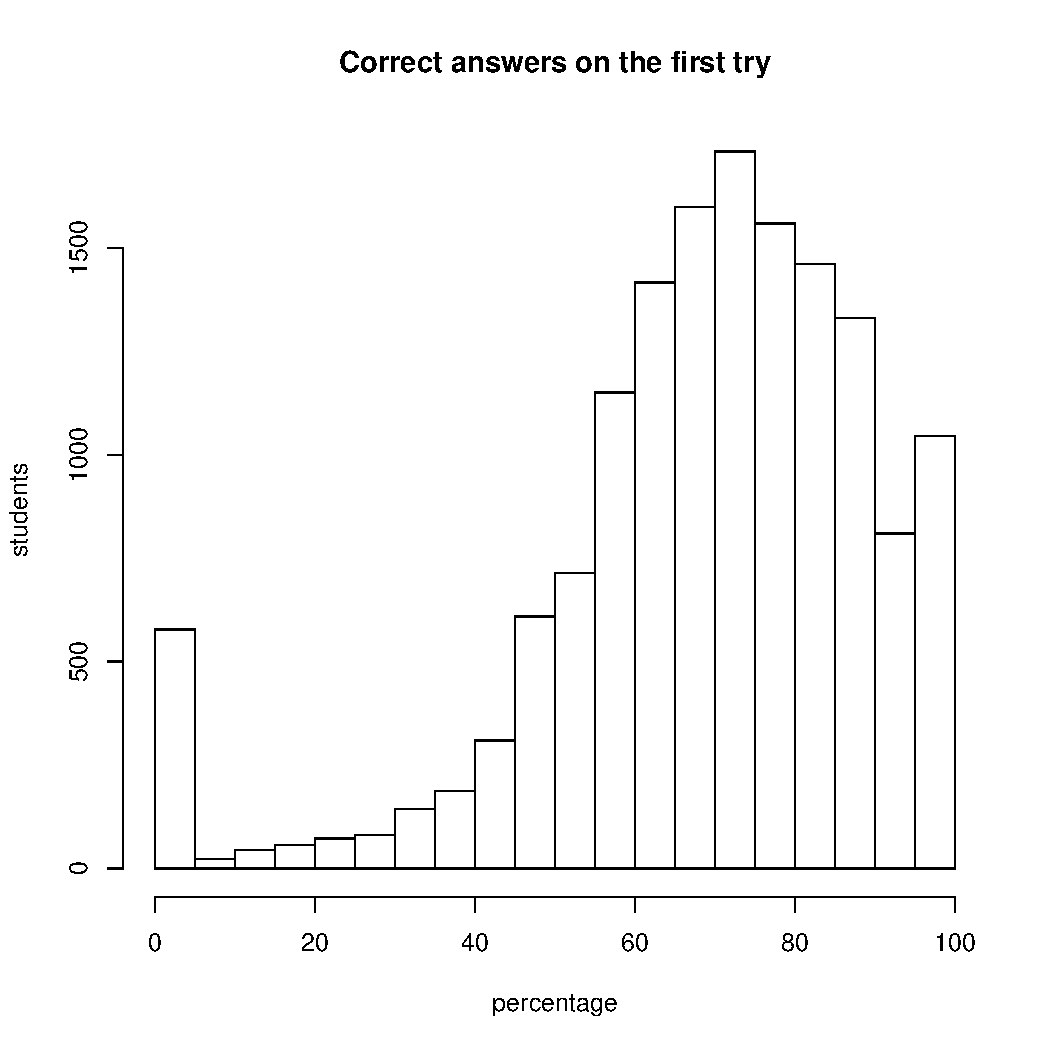
\includegraphics[height=0.9\textheight]{histogram-student-aces.pdf}
\end{center}
\end{frame}

\begin{frame}[nofills]
\vfill
\huge
point plotting \hfill 91\% correct \\
trig derivatives \hfill 57\% correct \\
related rates \hfill 35\% correct \\
\vfill
\end{frame}

% 92   93 0.08965517                 riemannSumIntegral
% 59   60 0.20494262                         chainRule2
% 79   80 0.22595420                  relatedRatesWhale
% 83   84 0.27857329         optimizationInstallingPipe
% 55   56 0.30439316                 productRuleTwoWays
% 87   88 0.30563862     optimizationPrescribingExtrema
% 85   86 0.31028887                  optimizationCubic
% 82   83 0.33673111      optimizationRectangleParabola
% 62   63 0.34052402                 tangentLineInverse
% 80   81 0.35260286         relatedRatesShadowBuilding
% 43   44 0.35597240                   linearTriangles1
% 100 101 0.37430168         areaValuedFunctionBehavior
% 41   42 0.38792559            differentiateUsingLimit
% 72   73 0.39896373                   inverseTrigDiff2
% 75   76 0.43156857                  relatedRatesBoats
% 40   41 0.43384836           continuityChooseConstant
% 73   74 0.43550071                 trigDifferentiate2
% 97   98 0.43797107                        eulerMethod
% 4     4 0.43958245                   derivativeOracle
% 12   12 0.45687926    functionTransformationPointwise
% 9     9 0.46231469                       limitsOracle
% 68   69 0.46735428                         chainRule1
% 44   45 0.47224174                   linearTriangles2
% 109 110 0.47511312                       smallRiemann
% 110 111 0.48148148                       variableSub1
% 25   25 0.48317297              limitsOracleGraphical
% 67   68 0.49526466          inverseFunctionExpression
% 88   89 0.50000000                   optimizationDrug
% 86   87 0.50304878                    optimizationBox
% 13   13 0.50542785                       limitCompute
% 38   38 0.51920422               tangentLineIdeaSlope
% 8     8 0.52440373                    bisectionOracle
% 74   75 0.52882612                    relatedRatesCow
% 23   23 0.54137951                     limitsSymbolic
% 90   91 0.54665530                      newtonsMethod
% 77   78 0.54864865                relatedRatesChronos
% 18   18 0.55172486                    limitsGraphical
% 53   54 0.56869433                quotientRuleCompute
% 28   28 0.57049331                  repeatedLinApprox
% 34   34 0.57350876                       linearOracle
% 70   71 0.57493979                  trigDifferentiate
% 71   72 0.58398649                   inverseTrigDiff1
% 37   37 0.58625020            limitsAtInfinityCompute
% 64   65 0.58883744          exponentiationDerivative2
% 24   24 0.58977061                   continuityOracle
% 78   79 0.59806068               relatedRatesBacteria
% 54   55 0.59896889                 quotientRulePoints
% 81   82 0.60579992                           lhopital
% 63   64 0.60823456                      ultimateWeek5
% 42   43 0.61939582              tangentLineIdeaSecant
% 35   35 0.61969493           limitsAtInfinitySymbolic
% 52   53 0.62804226                 productRuleCompute
% 89   90 0.63306763                       slopeFieldEQ
% 11   11 0.63504696      infiniteLimitsOracleGraphical
% 61   62 0.63514473             logarithmDifferentiate
% 45   46 0.63534266                  differentiability
% 84   85 0.64402985               optimizationPainting
% 95   96 0.64971751                         basicSigma
% 65   66 0.65187223                     chainRuleTable
% 36   36 0.66065978     comparingFunctionAndDerivative
% 31   31 0.66722664                       linearApprox
% 101 102 0.67799642           antiDerivativeBasicChain
% 3     3 0.67915697               intuitiveCurveSketch
% 10   10 0.68553342                       numChainRule
% 106 107 0.68800000                wiggleInputIntegral
% 96   97 0.69647059                     sigmaFormulas2
% 20   20 0.69652254               limitComputeInfinite
% 32   32 0.69674121            infiniteLimitsGraphical
% 19   19 0.70075262               infiniteLimitsOracle
% 76   77 0.70324383                 relatedRatesBubble
% 2     2 0.70713756                        approxDeriv
% 6     6 0.71997581          limitsAtInfinityGraphical
% 94   95 0.72097812 comparingFunctionAndAntiderivative
% 48   49 0.72228306                testingRandFunction
% 21   21 0.73713628                continuityGraphical
% 51   52 0.74414022                  curveSketchPoints
% 46   47 0.74669730               derivativeDefinition
% 16   16 0.74701441             limitsAtInfinityOracle
% 103 104 0.75182749 antiDerivativeAffineTransformation
% 58   59 0.75333333           inverseFunctionRulePoint
% 5     5 0.75797185                    limitsFactoring
% 27   27 0.75998364              isThisAFunctionPoints
% 39   40 0.76165665                    tangentLineIdea
% 22   22 0.76189465                evaluatingFunctions
% 30   30 0.76249565                     identifyMaxMin
% 60   61 0.79065276           exponentiationDerivative
% 50   51 0.79068279            differentiatePolynomial
% 98   99 0.79214195                     sigmaFormulas1
% 49   50 0.79285969                  productRulePoints
% 105 106 0.79321872       antidifferentiatePolynomials
% 107 108 0.79827089                estimatingIntegrals
% 57   58 0.79962980               secondDerivativeSign
% 33   33 0.83102657                  identifyConcavity
% 56   57 0.83879275    increaseDecreaseDerivativePoint
% 66   67 0.85415304              inverseFunctionPoints
% 7     7 0.86102934          continuityOracleGraphical
% 15   15 0.86919256                    pointOnFunction
% 99  100 0.87068025                         slopeField
% 104 105 0.87228167           antiDifferentiationBasic
% 47   48 0.87465480                     derivativeSign
% 26   26 0.87694914                     identifyPosNeg
% 102 103 0.87793427                antiDerivativeParts
% 1     1 0.89531053           identifyIncreaseDecrease
% 17   17 0.90256751                   abscissaOrdinate
% 14   14 0.91634648                          plotPoint
% 69   70 0.91945607          inverseFunctionPointGraph
% 29   29 0.93058247                   pointOnFunction2

\begin{frame}[nofills]
\begin{center}
\includegraphics[height=0.9\textheight]{covariance-first-twenty.pdf}
\end{center}
\end{frame}

\begin{frame}[nofills]
\begin{center}
\includegraphics[height=0.9\textheight]{covariance-first-twenty-highlighted.pdf}
\end{center}
\end{frame}

%6,limitsAtInfinityGraphical
%7,continuityOracleGraphical

\begin{frame}[nofills]
\Huge
\vfill
  Evolution requires \\
  \quad heritable variation.
\vfill\pause
  Unlike an offline course, \\
  \quad MOOCs offer this.
\vfill
\end{frame}


\setbackgroundpicturewhite{brownian-motion/brownian-motion-1.pdf}
\begin{frame}[nofills]
\null\vspace{1ex}
\Huge An analogy
\end{frame}
\setbackgroundpicturewhite{brownian-motion/brownian-motion-2.pdf}
\begin{frame}[nofills]
\end{frame}
\setbackgroundpicturewhite{brownian-motion/brownian-motion-3.pdf}
\begin{frame}[nofills]
\end{frame}
\setbackgroundpicturewhite{brownian-motion/brownian-motion-more-1.pdf}
\begin{frame}[nofills]
\end{frame}
\setbackgroundpicturewhite{brownian-motion/brownian-motion-more-2.pdf}
\begin{frame}[nofills]
\end{frame}
\setbackgroundpicturewhite{brownian-motion/brownian-motion-more-3.pdf}
\begin{frame}[nofills]
\end{frame}
\setbackgroundpicturewhite{brownian-motion/brownian-motion-more-4.pdf}
\begin{frame}[nofills]
\end{frame}
\setbackgroundpicturewhite{brownian-motion/brownian-motion-more-5.pdf}
\begin{frame}[nofills]
\end{frame}
\setbackgroundpicturewhite{brownian-motion/brownian-motion-more-5.pdf}
\begin{frame}[nofills]
\Huge Teaching without data? \\

\vfill

\quad A random walk.
\vspace{1in}
\end{frame}

\setbackgroundpicturewhite{brownian-motion/brownian-motion-weighted-1.pdf}
\begin{frame}[nofills]
\null\vspace{1ex}
\Huge But with feedback?
\end{frame}
\setbackgroundpicturewhite{brownian-motion/brownian-motion-weighted-2.pdf}
\begin{frame}[nofills]
\end{frame}
\setbackgroundpicturewhite{brownian-motion/brownian-motion-weighted-3.pdf}
\begin{frame}[nofills]
\end{frame}
\setbackgroundpicturewhite{brownian-motion/brownian-motion-weighted-more-1.pdf}
\begin{frame}[nofills]
\end{frame}
\setbackgroundpicturewhite{brownian-motion/brownian-motion-weighted-more-2.pdf}
\begin{frame}[nofills]
\end{frame}
\setbackgroundpicturewhite{brownian-motion/brownian-motion-weighted-more-3.pdf}
\begin{frame}[nofills]
\end{frame}
\setbackgroundpicturewhite{brownian-motion/brownian-motion-weighted-more-4.pdf}
\begin{frame}[nofills]
\end{frame}
\setbackgroundpicturewhite{brownian-motion/brownian-motion-weighted-more-5.pdf}
\begin{frame}[nofills]
\end{frame}
\setbackgroundpicturewhite{brownian-motion/brownian-motion-weighted-more-5.pdf}
\begin{frame}[nofills]
\Huge Online is not the point.
\vfill
Data-driven feedback is.
\vspace{1cm}
\end{frame}

\setbackgroundpicturewhite{brownian-motion/brownian-motion-together.pdf}
\begin{frame}[nofills]
\Huge \uncover<2->{\color{blue}{MOOCs will improve.}}
\vfill
\uncover<3->{\color{red}{Will the University?}}
\end{frame}




 %%%%%%%%%%%%%%%%%%%%%%%%%%%%%%%%%%%%%%%%%%%%%%%%%%%%%%%%%%%%%%%%
 \clearbackgroundpicture
 \begin{frame}[nofills]
   \vfill
   \begin{center}
   \Huge
    \scalebox{1.5}{\textbf{Thank You}}
   \end{center}
   \vfill
   \includegraphics[width=1in]{cc-logo.pdf}
   \hfill\footnotesize\scalebox{0.9}{licensed for reuse under a Creative Commons BY-NC-ND License}
   \null
 \end{frame}

\end{document}
